\subsection{Image Meter}

\subsubsection{Vorstellung}
Die App \im{} von \emph{Dirk Farin} hat zur Zeit des Downloads (20. Januar 2018) bei insgesamt 2 764 abgegeben Bewertungen eine durchschnittliche Bewertung von 3,9 von 5 Sternen im Google Play-Store \citep{FarinIM}.
Hierbei haben 72\% (1978) der Bewertungen vier oder fünf, und nur 28\% (786) 3 oder weniger Sterne.
Dies ist eine überdurchschnittlich hohe Bewertung, und macht die App zu einer der Beliebtesten unter dem Suchbegriff ``Aufmaße''.
Der Entwickler selbst beschreibt die App im Play-Store wie folgt \citep{FarinIM}:

\begin{quote}
  ``ImageMeter erlaubt das Beschriften Ihrer Fotos mit Längen-, Winkel- und Flächenmaßen sowie Text.
  Das ist viel einfacher und anschaulicher als aufwändig eine Skizze zu zeichnen.''
\end{quote}

\noindent
Beim Start der App wird dem Benutzer der sogenannte ``Tipp des Tages'' angezeigt.

\begin{wrapfigure}{R}{0.5\textwidth}
  \centering
  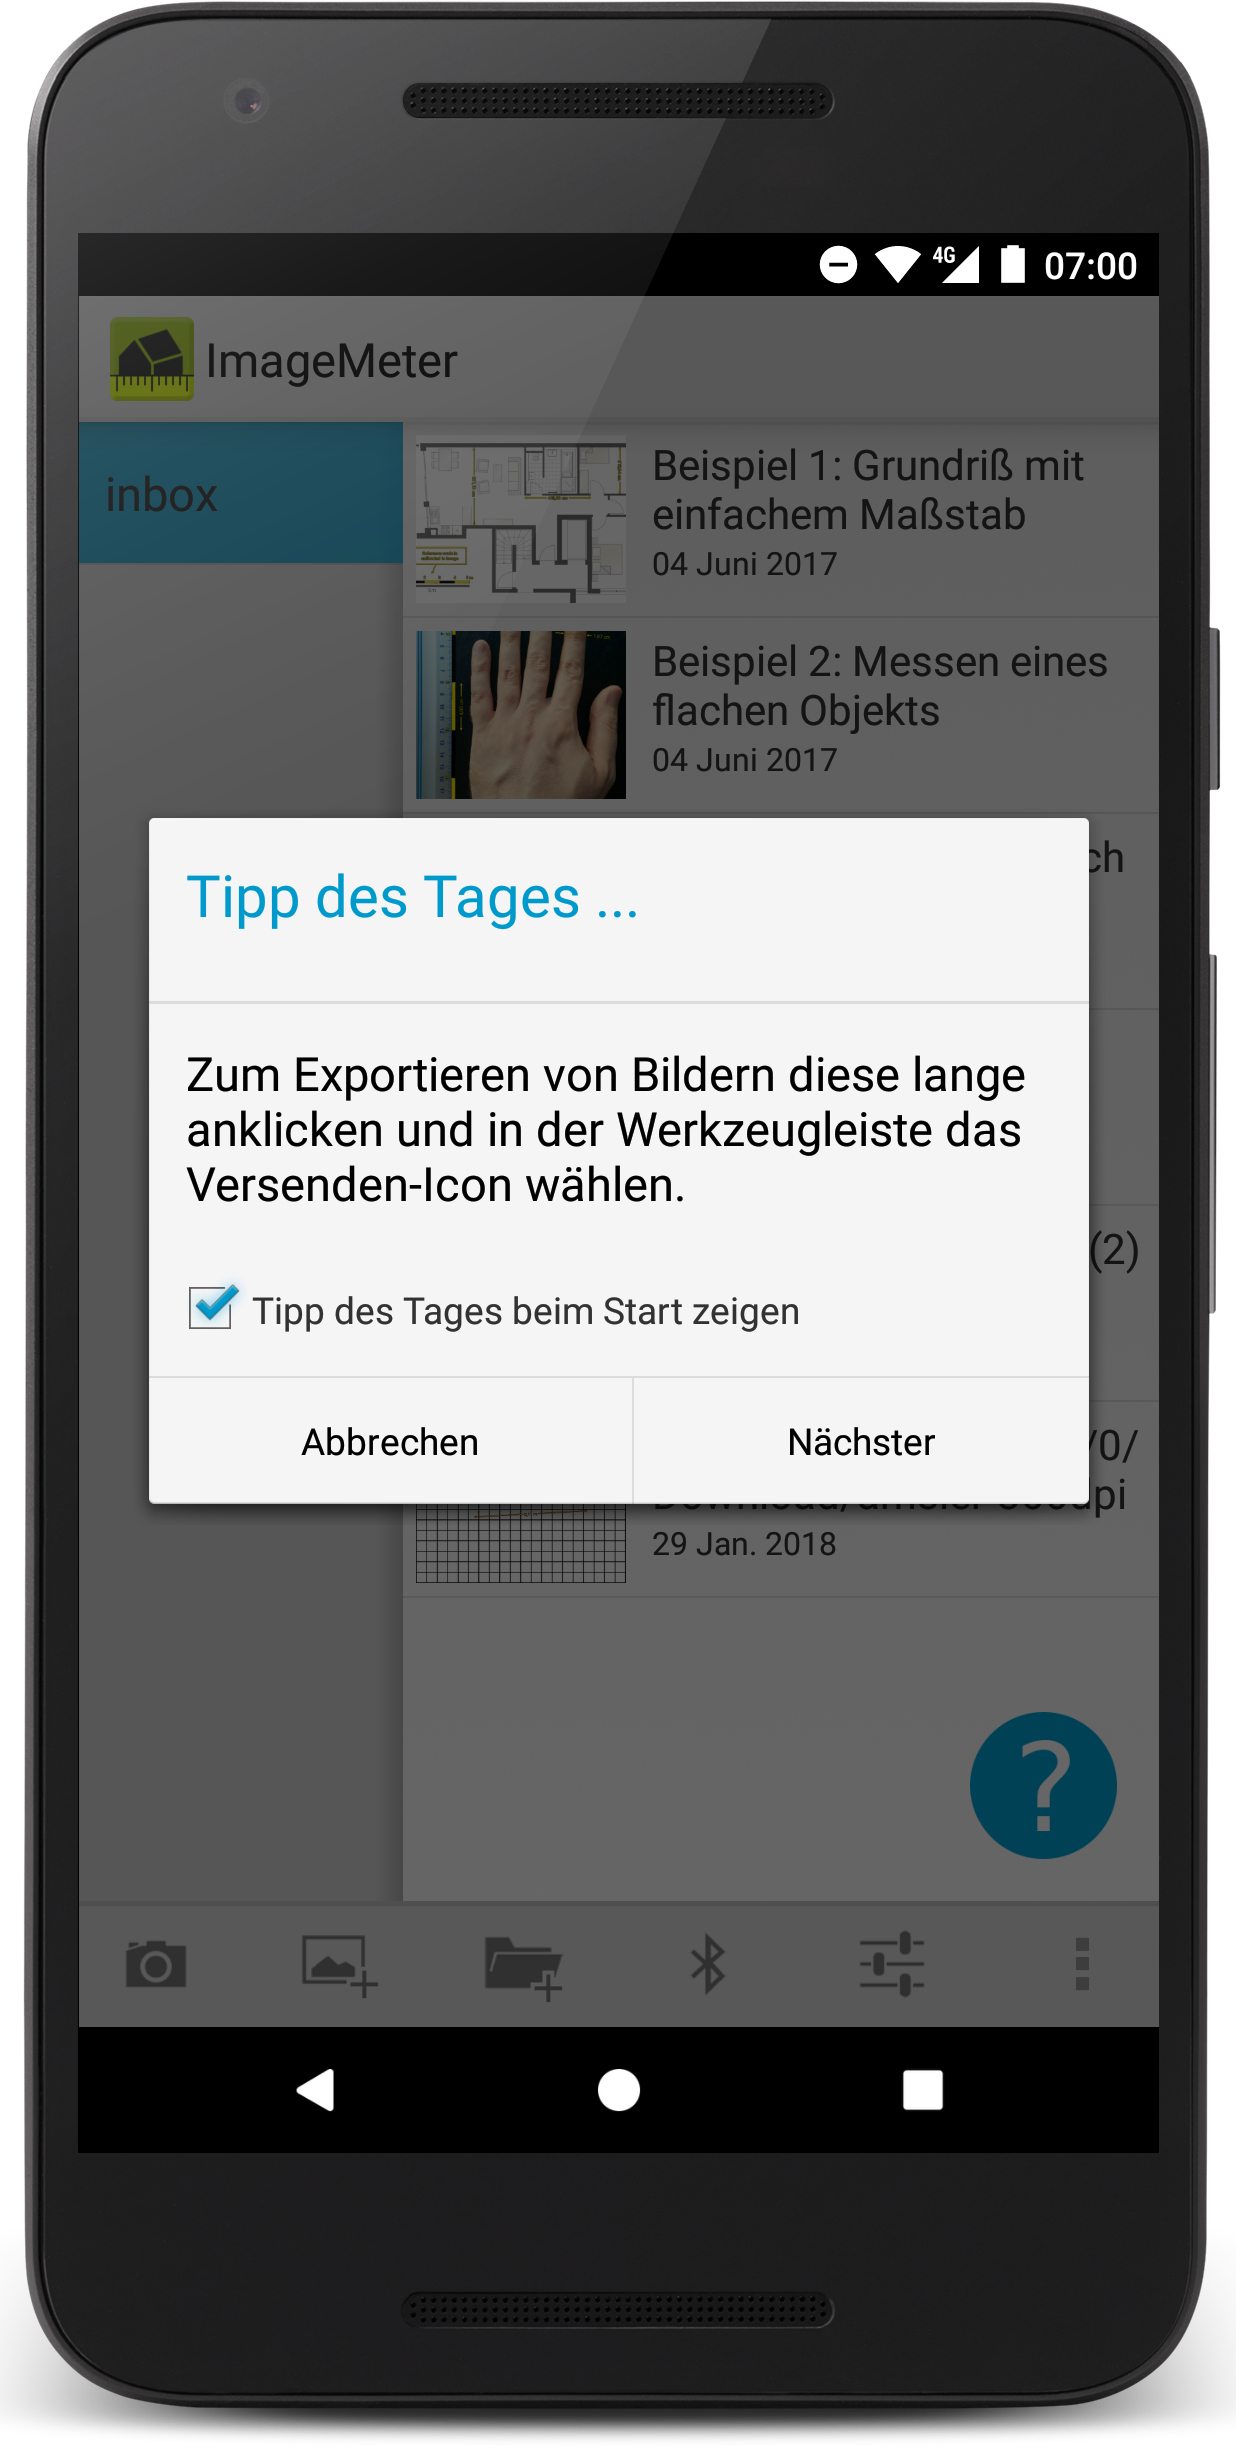
\includegraphics[keepaspectratio, width=0.5\textwidth]{image_meter/tip}
  \caption{``Tipp des Tages'' beim Start der App}
  \label{fig:imtip}
\end{wrapfigure}

Dieser enthält Informationen zu bestimmten Funktionen der App, wie zum Beispiel dem Exportieren von Bildern (siehe \autoref{fig:imtip}).
Hier hat der Nutzer die Möglichkeit sich weitere Tipps anzusehen, oder diese durch das Entfernen des Hakens in der Checkbox ``Tipp des Tages beim Start zeigen'' dauerhaft zu deaktivieren. \\

Sobald der Dialog zum ``Tipp des Tages'' geschlossen wurde, bietet sich über die Statusleiste am unteren Bildschirmrand die Möglichkeit, ein neues Bild aufzunehmen, oder direkt eines aus der Galerie zu importieren (siehe \autoref{fig:immenu}). \\

Das ausgewählte Bild wird nach erfolgreichem Import in die App im Hauptmenü in einer Liste mit alleren weiteren Bildern angezeigt.
Hier gelangt der Benutzer durch einen Klick auf das gewünschte Bild in eine neue Bildschirmoberfläche, in der das Bild beschriftet werden kann (siehe \autoref{fig:imdraw}).
In dieser Oberfläche wird dem Nutzer das zuvor ausgewählte Bild und eine neue Statusleiste am unteren Bildschirm angezeigt.
Oberhalb der Statusleiste befindet sich ein ``Floating Action Button'' (\emph{FAB}), der durch ein Fragezeichen-Icon gekennzeichnet ist.
Der \emph{FAB} öffnet beim Klick auf sich eine separate Hilfe-Seite, in der häufig gestellte Fragen und deren Antworten zu den Funktionen der App beschrieben stehen. \\

Zusätzlich zu dieser Hilfestellung, wird dem Benutzer beim Auswählen des Zeichen-Modus ein erklärender Text über der Statusleiste angezeigt (siehe \autoref{fig:imdraw}).
Dieser beschreibt genau, welche Aktion der Nutzer im aktuellen Systemzustand durchführen kann bzw. soll. \\

\begin{figure}[h]
  \centering
  \begin{subfigure}[t]{0.4\textwidth}
    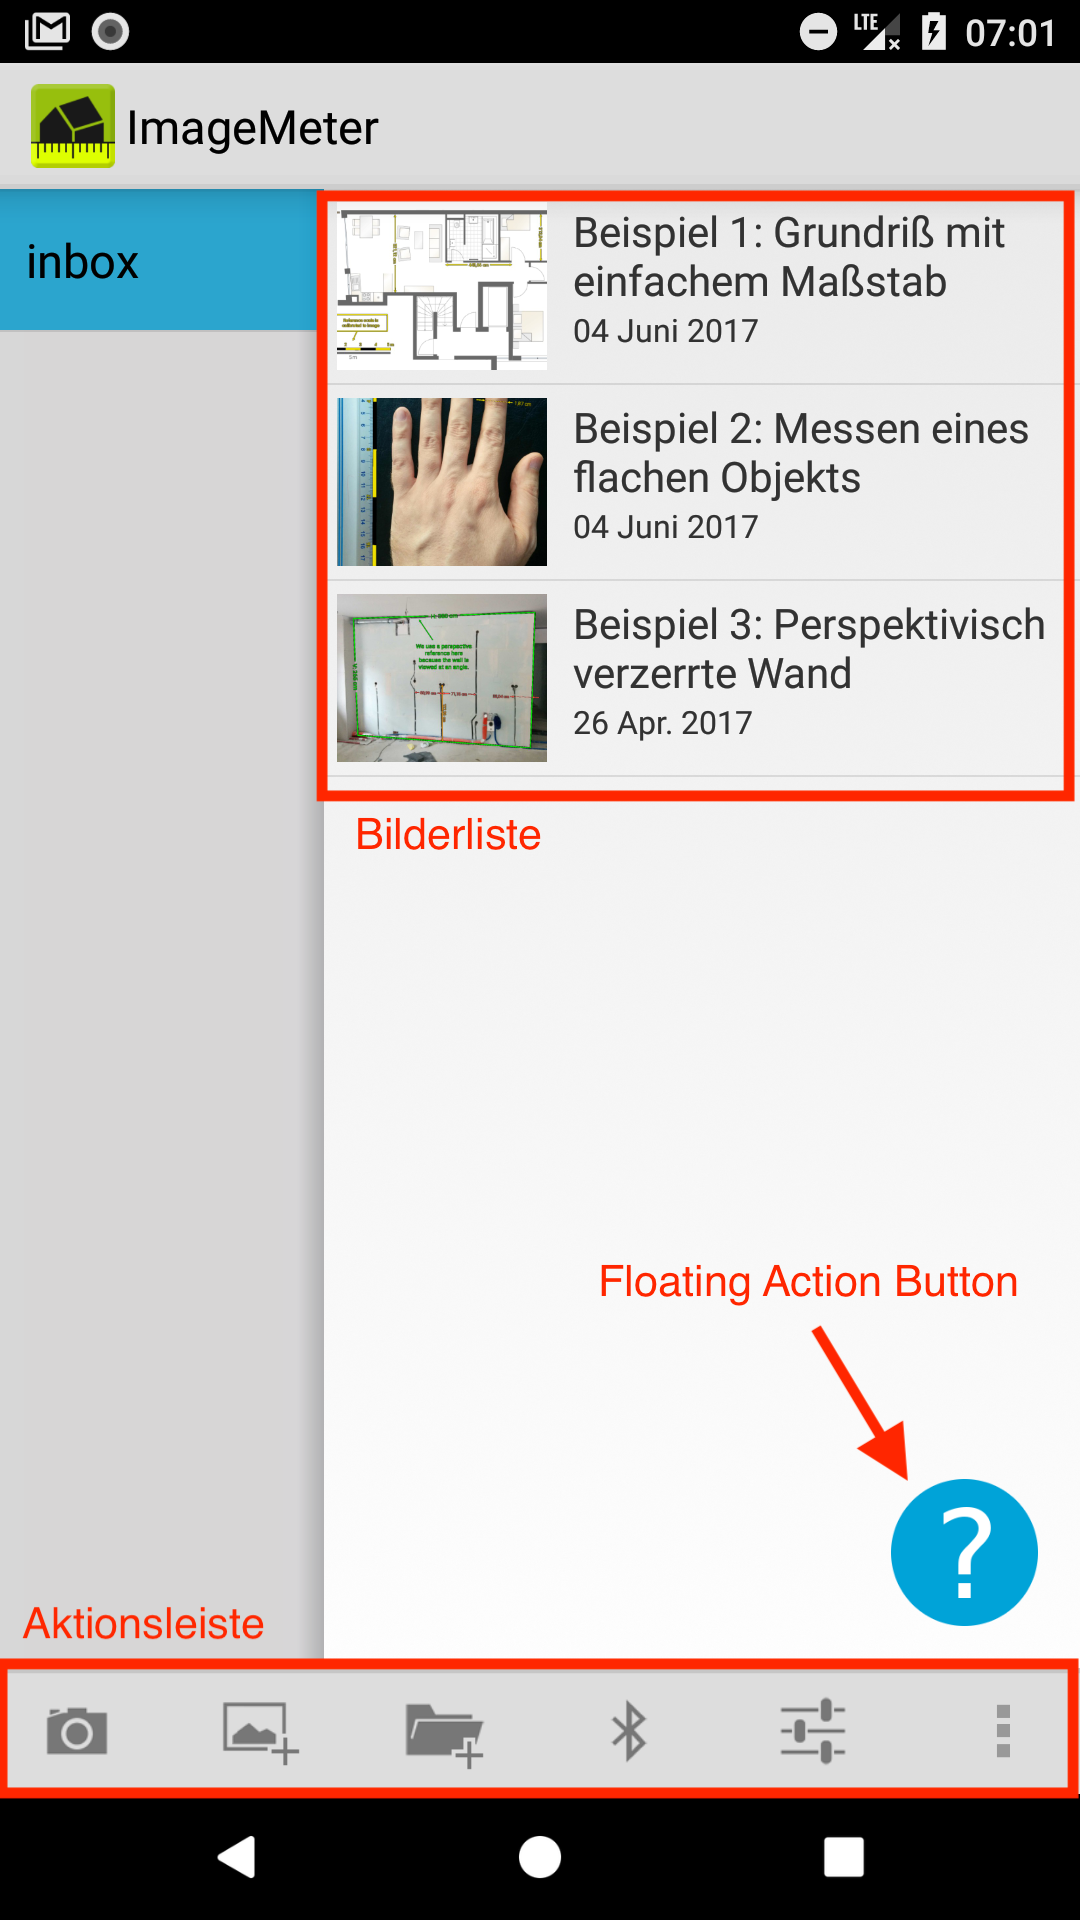
\includegraphics[keepaspectratio, width=\textwidth]{image_meter/menu}
    \caption{Hauptansicht der App}
    \label{fig:immenu}	
  \end{subfigure}
  \begin{subfigure}[t]{0.4\textwidth}
    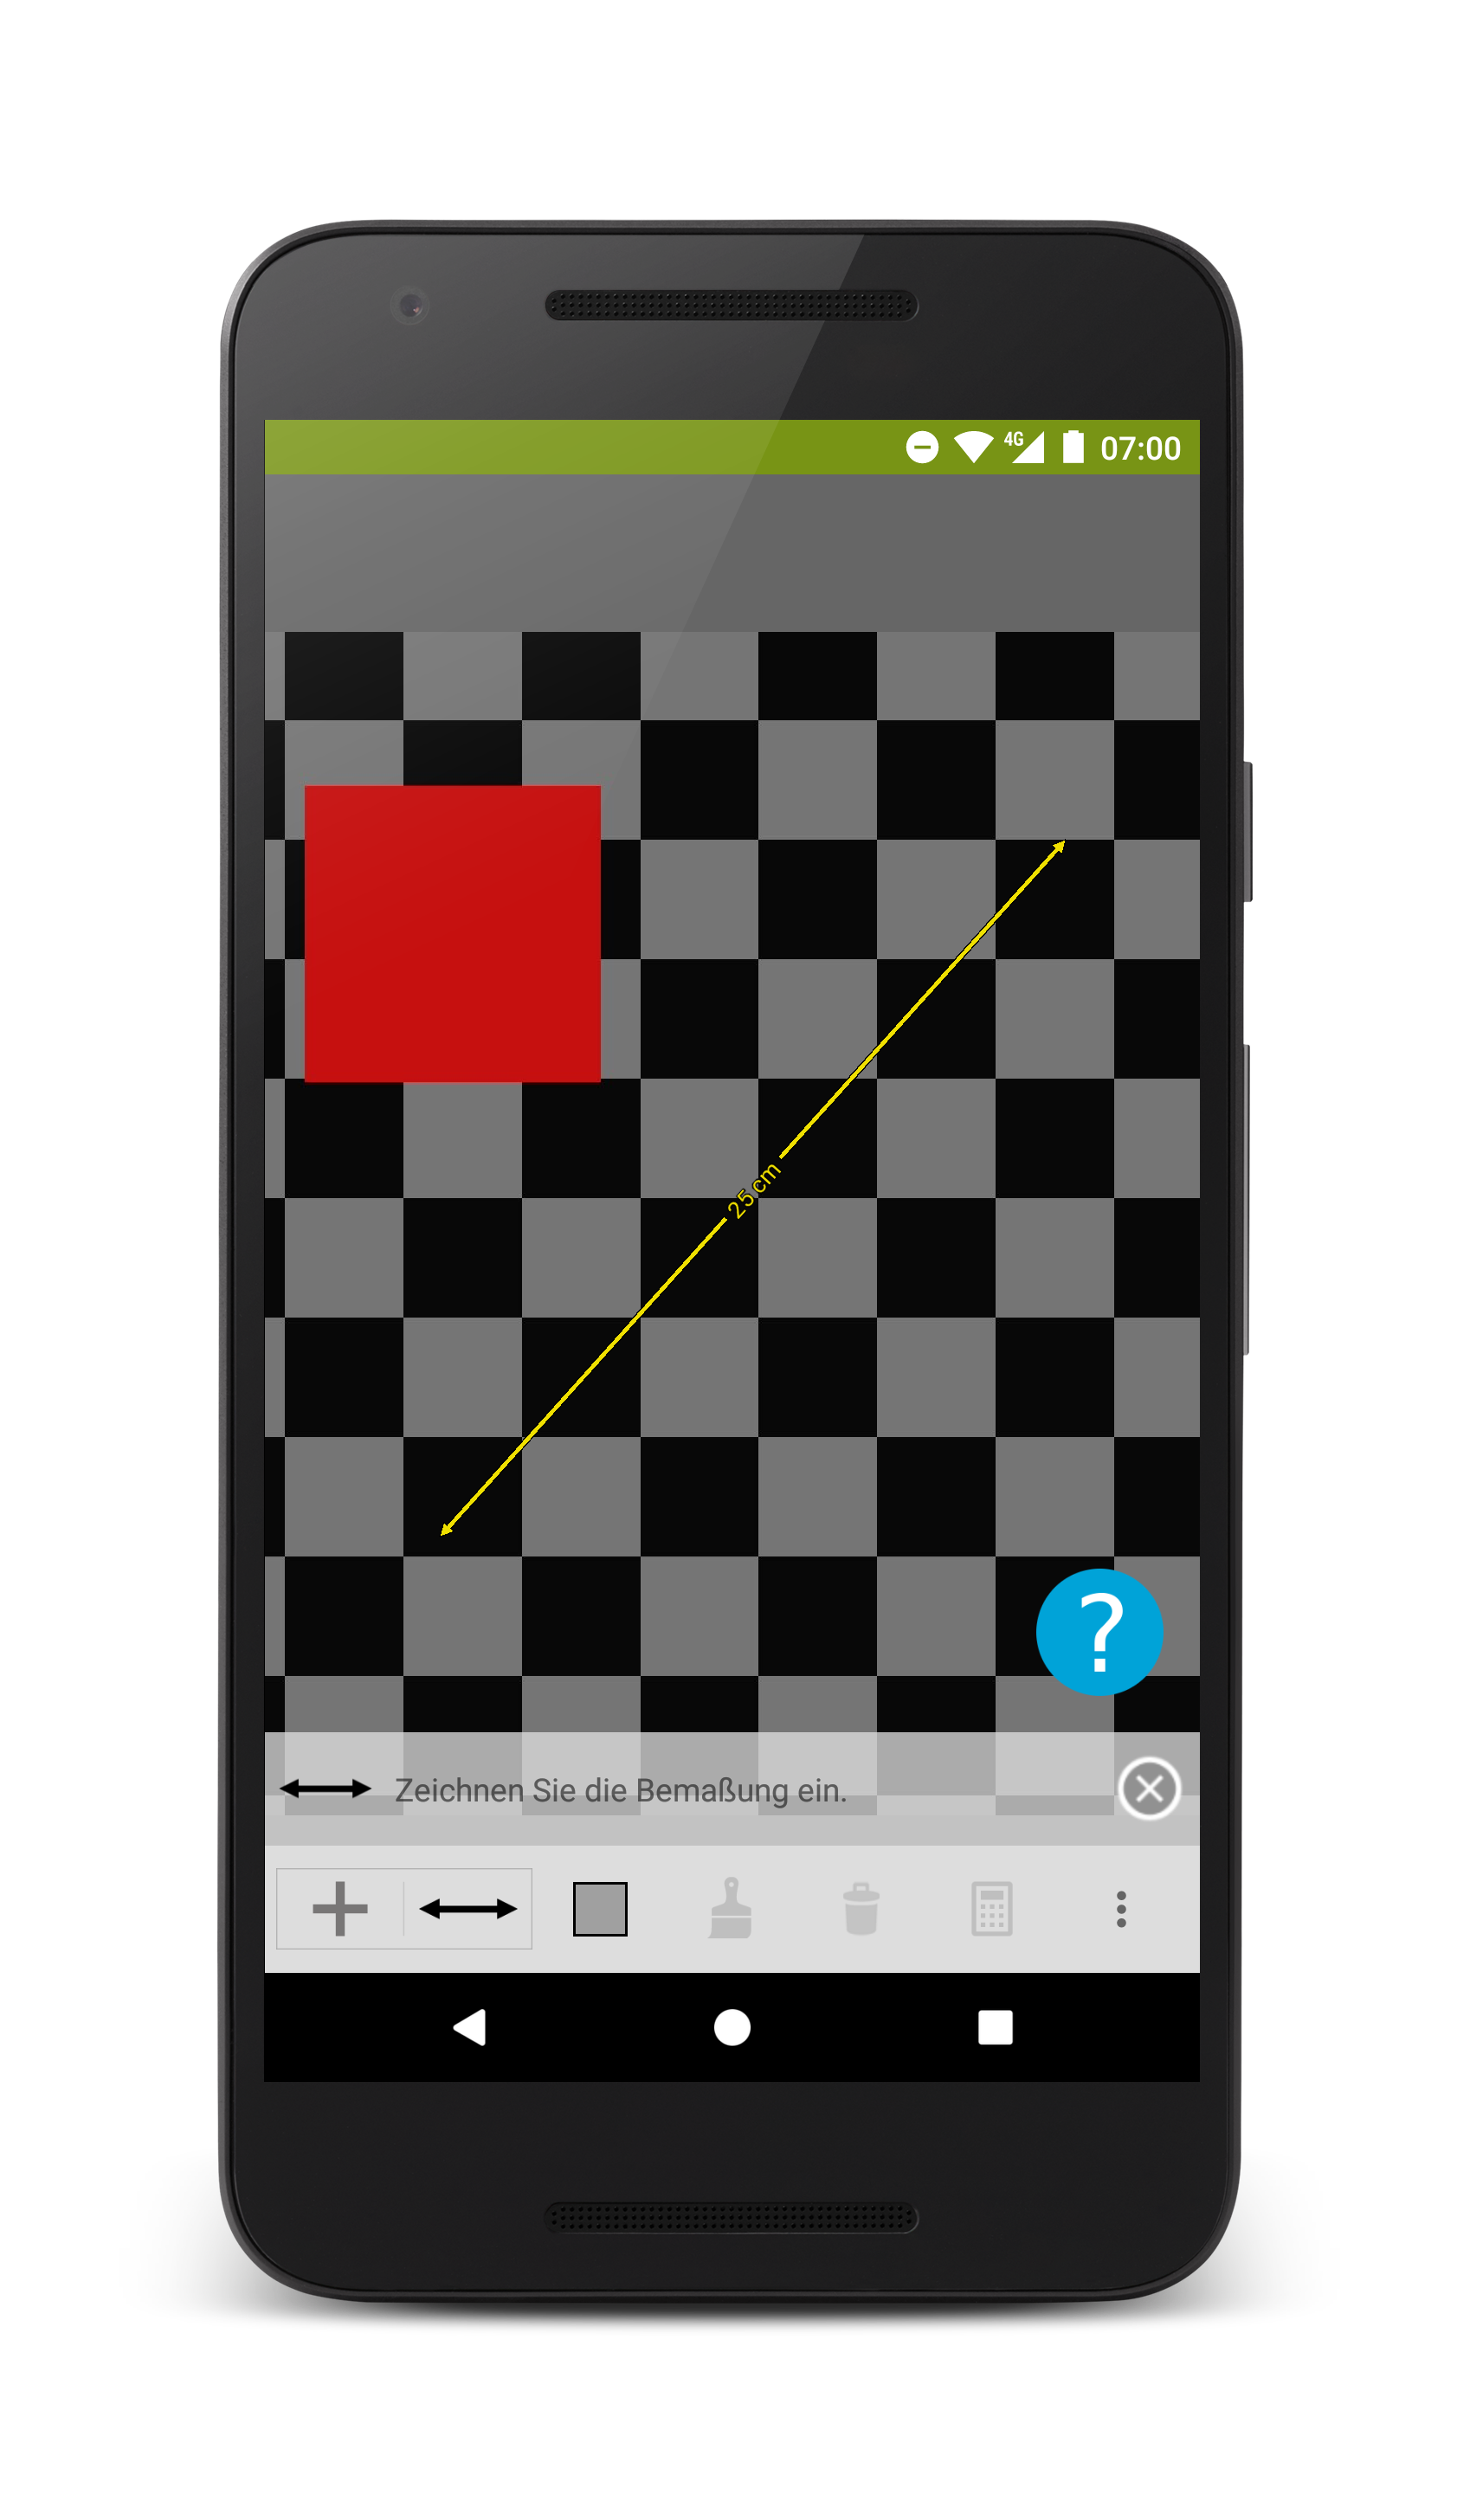
\includegraphics[keepaspectratio, width=\textwidth]{image_meter/draw}
    \caption{Aufmaße-Funktion mit eingezeichneter Form} 
    \label{fig:imdraw}	
  \end{subfigure}
  \caption{\im{} nach dem Start der App und in der Aufmaß-Funktion}
\end{figure}

\noindent
Die Statusleiste bietet dem Nutzer außerdem die Möglichkeit, die gewünschte Form und deren Farbe festzulegen.
Die Farbe bereits eingezeichneter Formen kann auch noch im Nachhinein angepasst werden.
Zu jeder Zeit sind nur die Funktionen in der Statusleiste auswählbar, die im aktuellen Systemzustand durchführbar sind.
So ist bspw. das Löschen von Formen nur dann möglich, wenn zuvor eine Form markiert wurde. \\

Insgesamt kann der Nutzer aus bis zu sieben verschiedene Formen (zehn in der Pro-Version) frei auswählen.
Unter diesen sieben Formen der Free-Version befinden sich auch zwei Referenz-Formen.
Diese können dazu genutzt werden, um Referenzlängen im Bild festzulegen, und ermöglichen so, dass alle nachträglich eingezeichneten Formen automatisch mit Messwerten versehen werden. \\

Eine Undo- bzw. Redo-Funktion ist über das \emph{Overflow-Menü} in der Statusleiste erreichbar.
Hierdurch können ausgeführte Aktionen rückgängig gemacht oder wiederholt werden. \\

Auch in dieser App lassen sich gespeicherte Bilder zu einem späteren Zeitpunkt weiter bearbeiten.
Außerdem können mehrere Bilder gleichzeitig zusammen in einer \emph{PDF} exportiert werden.

\subsubsection{Evaluation}\label{subsec:imeva}
Hilfe und Dokumentation (Nielsen~\autoref{itm:N10}) werden in dieser App in Form des ``Tipp des Tages'' (siehe \autoref{fig:imtip}) und die dedizierte Hilfe-Oberfläche bereits gestellt.

\begin{wrapfigure}{R}{0.5\textwidth}
  \centering
  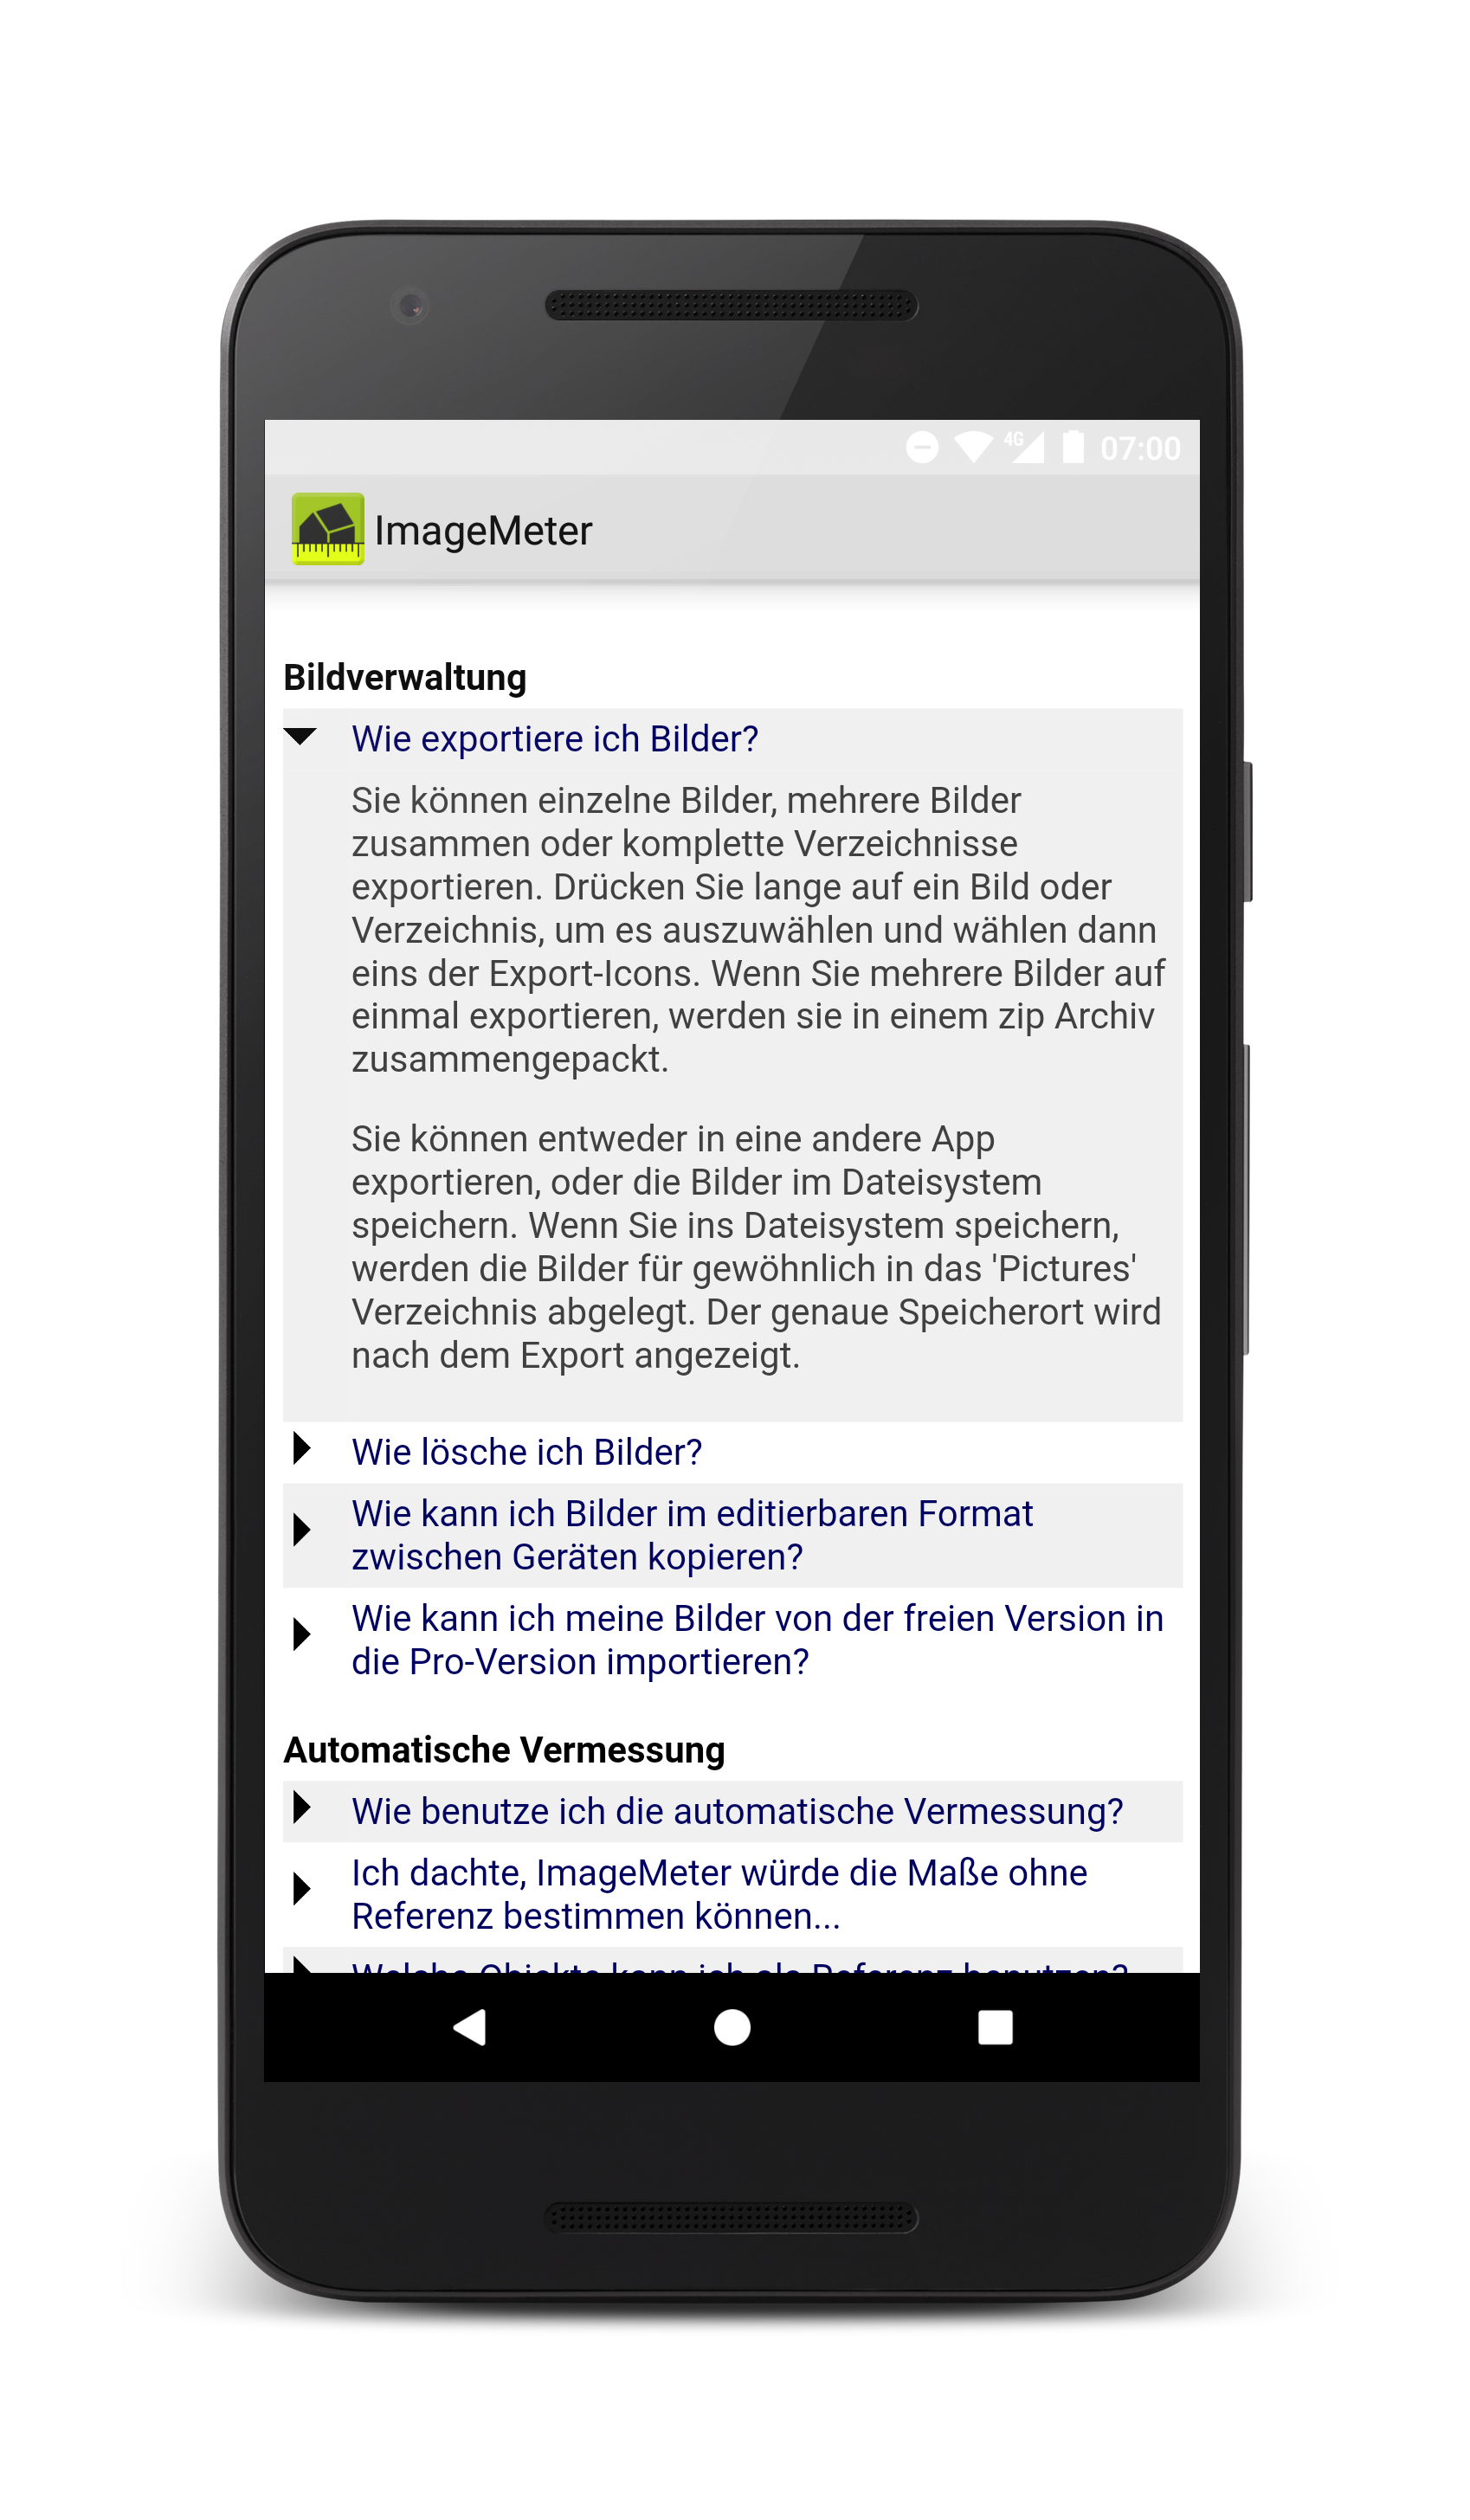
\includegraphics[keepaspectratio, width=0.5\textwidth]{image_meter/faq}
  \caption{Hilfeoberfläche der App}
  \label{fig:imfaq}
\end{wrapfigure}

Hierbei bietet die Hilfe-Oberfläche Antworten auf eine vorgegebene Menge an Fragen zu den verschiedenen Funktionen der App an (siehe \autoref{fig:imfaq}). \\

Die Statusleiste zeigt zu jedem Zeitpunkt den ausgewählten Modus und die ausführbaren Aktionen an.
Hierdurch gibt die App dem Nutzer eine angemessene und verständliche Rückmeldung über den aktuellen Systemzustand der App (Nielsen~\autoref{itm:N1} \& \autoref{itm:N5}). \\

Formen können, nachdem sie in das Bild gezeichnet wurden, zu einem späteren Zeitpunkt in ihrer Farbe und Größe verändert werden.
Zusätzlich dazu gibt es in den Einstellungen der App weitere Optionen, um die App an die eigenen Bedürfnisse anzupassen.
So kann zum Beispiel eingestellt werden, ob Maßeinheiten angezeigt werden sollen, welche metrischen Einheiten benutzt werden sollen, oder wie viele Dezimalstellen für Messwerte verwendet werden solle.
Dies erlaubt nicht nur eine flexible Benutzung der App, sondern kann gleichzeitig zu einer Effizienzsteigerung führen, da die App nur einmal zu Beginn der Benutzung konfiguriert werden muss (Nielsten~\autoref{itm:N7}) \\

Die App versucht Situationen, in denen Fehler auftreten könnten, präventiv zu vermeiden.
Hierzu werden Aktionen, die beim Ausführen im aktuellen Systemzustand zu einem Fehler führen würden, ausgegraut und sind nicht auswählbar (Nielsen~\autoref{itm:N5} \& \autoref{itm:N9}).

\begin{wrapfigure}{R}{0.5\textwidth}
  \centering
  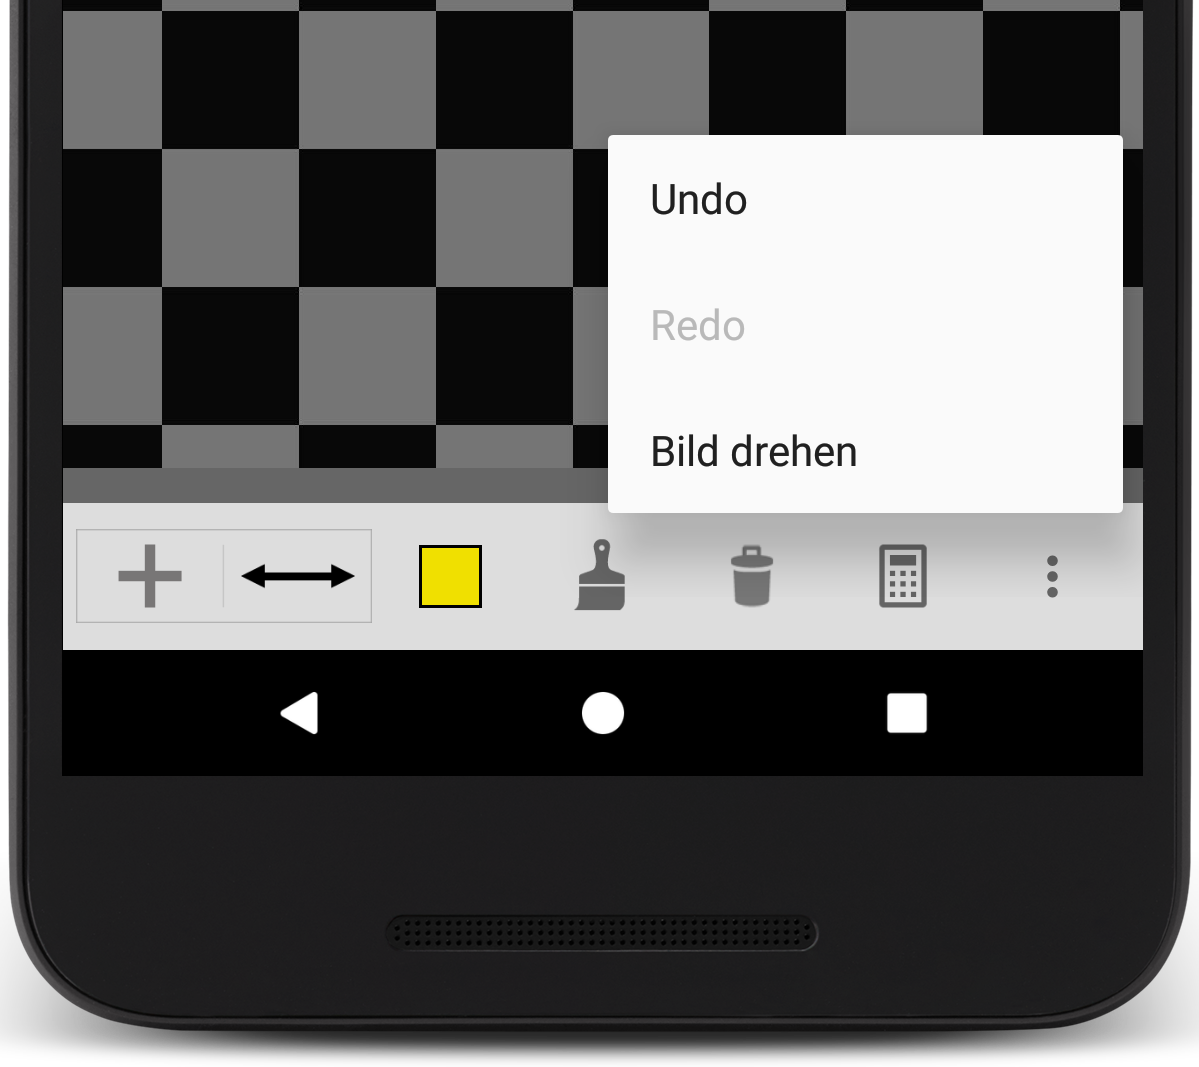
\includegraphics[keepaspectratio, width=0.5\textwidth]{image_meter/bar}
  \caption{Statusleiste in der Aufmaßfunktion}
  \label{fig:imbar}
\end{wrapfigure}

Das Ausgrauen der unbenutzbaren Icons kann jedoch in Kombination mit den anderen verwendeten Farben in der Statusleiste zu Verwirrung führen.
So werden hier zwei verschiedene Grautöne benutzt, die sich nur minimal unterscheiden (siehe \autoref{fig:imbar}). 
\todo{bisschen mehr hierzu} \\

Über einen Undo- bzw. Redo-Button hat der Benutzer die Möglichkeit, fehlerhafte Eingaben zu verbessern, oder Aktionen zu wiederholen (Nielsen \autoref{itm:N3}).
Bei der Benutzung im Hochformat sind beide Buttons jedoch nicht sichtbar, da sie in dem \emph{Overflow-Menü} an der rechten Seite der Statusleiste versteckt sind (siehe \autoref{fig:imbar}).
Der Benutzer ist hier also darauf angewiesen, das \emph{Overflow-Menü} anzuklicken, um zu wissen, dass sich dort die Optionen zum Undo bzw. Redo befinden.
Generell fühlt sich die Statusleiste mit den sieben Icons (inklusive \emph{Overflow-Menü}) zu überladen an.
Hier wäre die Verwendung einer zusätzlichen Menüleiste sinnvoll, die einen Teil der Icons übernimmt. \\
\todo{anders schreiben}

Ein positiver Aspekt dagegen liegt beim adäquaten Umgang mit Unterbrechungen, sowie der Unterstützung verschiedener Bildschirmausrichtungen (Nielsen~\autoref{itm:N11} \& \autoref{itm:N15}).
Beim Pausieren und Drehen der App gehen keine Informationen, wie bereits eingezeichnete Formen oder eingetragene Messwerte verloren, und das Bild bleibt stets in der erwarteten Ausrichtung. 

\begin{wrapfigure}{R}{0.5\textwidth}
  \centering
  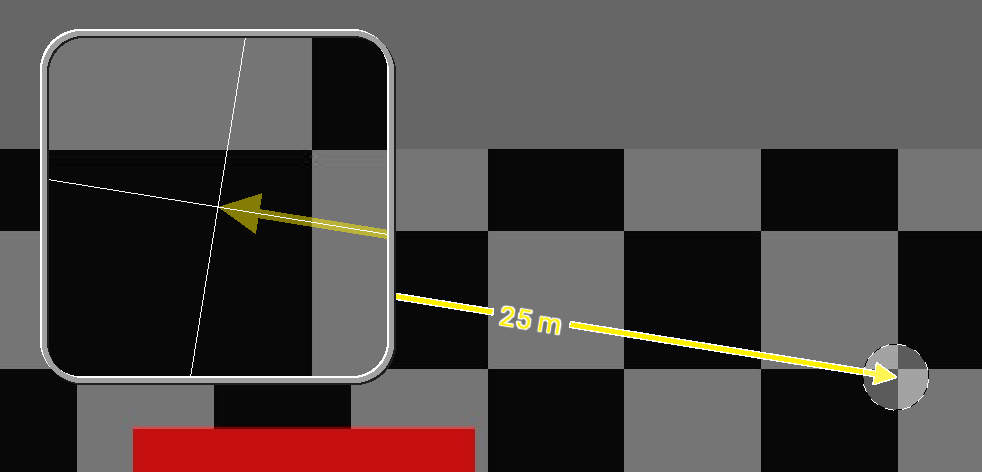
\includegraphics[keepaspectratio, width=0.5\textwidth]{image_meter/lensebug}
  \caption{Zoom-Linse verdeckt Zeichenbereich}
  \label{fig:imlense}
\end{wrapfigure}

Hinzukommend wird der zusätzliche Bildschirmplatz der sich im Querformat ergibt genutzt, um alle Elemente der Statusleiste anzuzeigen, ohne Aktionen im Overflow-Menü zu verstecken. \\

Eine positive Benutzererfahrung ergibt sich aus der einfachen und effizienten einhändigen Handhabung in Kombination mit einer fehlerfreien Gesten-Unterstützung zur Navigation im Bild. (Nielsen~\autoref{itm:N13}, \autoref{itm:N16} \& \autoref{itm:N17}). \\

Außerdem bedient sich auch diese App beim Zeichnen von Formen einer Zoom-Linse, welche den Bereich um die Fingerposition vergößert darstellt.
Negativ fällt bei der Umsetzung dieser Funktion jedoch auf, dass die Zoom-Linse statisch in der oberen linken Ecke angezeigt wird, und sich bei Kollision mit dem Zeichenfinger nicht bewegt.
Dies kann dazu führen, dass der gezoomte Bereich beim Zeichnen die Form verdeckt und seine eigentlichen Aufgabe als Hilfestellung zur genaueren und schnelleren Zeichnung verfehlt (siehe \autoref{fig:imlense}). \\

Die App ermöglicht das Teilen von vorhandenen Bildern in diese, bietet beim Exportieren jedoch keine Möglichkeit die eingetragenen Messwerte als Meta-Daten beizubehalten.
So wäre es zwar möglich, Bilder aus der bestehenden Android-App an \im{} zu teilen, diese zu bearbeiten und anschließend abzuspeichern. 
Aber es gäbe keine Möglichkeit aus der bestehenden Android-App auf die eingetragenen Messwerte zuzugreifen, und diese für einen nachgeschalteten Diesnt aufzubereiten. \\

Zusammenfassend kann gesagt werden, dass die App \im{} von \emph{Dirk Farin} die Nielsen-Heuristiken überwiegend positive erfüllt.
Die versteckten Undo/Redo-Funktionalität und die Verwirrung des Nutzers durch die Verwendung ähnlicher Grautöne für unterschiedliche Aktionen in der Statsubar sind bei der Evaluation als Negativaspekte identifiziert worden.
Besonders diese beiden Punkte in Kombination mit der fehldenden Einführung bzw. Hilfe-Stellung beim ersten Start der Aufmaß-Funktion, wirken sich negativ auf die initiale Benutzererfahrung der App aus.
So muss der Benutzer, falls sich Fragen während des Einzeichnens von Formen ergeben, die aktuelle Oberfläche verlassen, in eine andere Oberfläche wechseln, und dort die passende Frage suchen. 

Hierdurch können Fehler entstehen, die mit der Nutzung einer Android-App für die Aufmaßerfassung verhindert werden sollten.
